\documentclass{article}%
\usepackage[T1]{fontenc}%
\usepackage[utf8]{inputenc}%
\usepackage{lmodern}%
\usepackage{textcomp}%
\usepackage{lastpage}%
\usepackage[head=40pt,margin=0.5in,bottom=0.6in]{geometry}%
\usepackage{graphicx}%
%
\title{\textbf{Primero Justicia: Concejal Fernando Albán fue asesinado en la sede del Sebin}}%
\author{COMUNICADO}%
\date{08/10/2018}%
%
\begin{document}%
\normalsize%
\maketitle%
\textbf{URL: }%
http://www.eluniversal.com/sucesos/22693/primero{-}justicia{-}concejal{-}fernando{-}alban{-}fue{-}asesinado{-}en{-}la{-}sede{-}del{-}sebin\newline%
%
\textbf{Periodico: }%
EU, %
ID: %
22693, %
Seccion: %
sucesos\newline%
%
\textbf{Palabras Claves: }%
NO\_TIENE\newline%
%
\textbf{Derecho: }%
1.1, %
Otros Derechos: %
1.2, %
Sub Derechos: %
1.1.1.3, 1.2.2\newline%
%
\textbf{EP: }%
NO\newline%
\newline%
%
\textbf{\textit{En un comunicado, el partido político descartó  el suicidio y responsabilizó a los cuerpos de seguridad y al gobierno. Exigen que el hecho que ocurrió este lunes no quede impune}}%
\newline%
\newline%
%
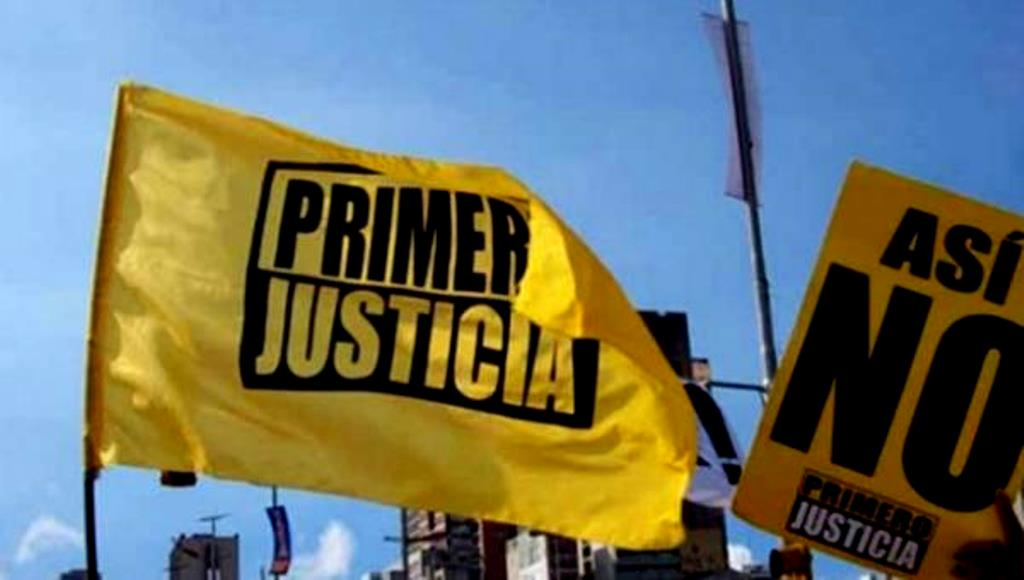
\includegraphics[width=300px]{149.jpg}%
\newline%
%
Caracas.{-} Tras conocerse la muerte del concejal Fernando Albán, la dirección nacional del partido Primero Justicia emitió el siguiente comunicado:%
\newline%
%
"Con profundo dolor y sed de justicia nos dirigimos al pueblo de Venezuela, especialmente a los justicieros de todo el país, para informar que el concejal Fernando Albán murió asesinado en manos del régimen de Nicolás Maduro en el SEBIN de Plaza Venezuela. Tarek William Saab, un reconocido verdugo de la dictadura, informó un supuesto suicidio. Pero los compañeros de lucha y amigos de Fernando Albán sabemos que era un hombre fuerte y de profundos valores cristianos. Responsabilizamos a Nicolás Maduro y a su régimen torturador de lo ocurrido. Exigimos la verdad de las cosas y declaramos que esta dolorosa situación demuestra lo peor de la dictadura: un sistema de muerte que penetra en la conciencia de quienes defendemos la libertad en Venezuela. Este hecho debe remover la opinión pública nacional e internacional y procederemos a todos los organismos nacionales e internacionales para establecer responsabilidades y castigar a todos los culpables, comenzando por Nicolás Maduro.\newline%
\newline%
Exigimos justicia y pedimos oraciones para su alma. En breve ofrecemos más información".%
\newline%
%
\end{document}